\documentclass[tikz,border=9pt,12pt]{standalone}
\usepackage{amsmath,amssymb}
\usetikzlibrary{arrows.meta,calc}
\tikzset{every node/.style={text=black,font=\normalsize},axis/.style={-{Stealth[length=2mm]},black!65,thin},vec/.style={-{Stealth[length=2.8mm]},line width=1.3pt,blue!70!black},lab/.style={fill=white,inner sep=2pt}}
\begin{document}
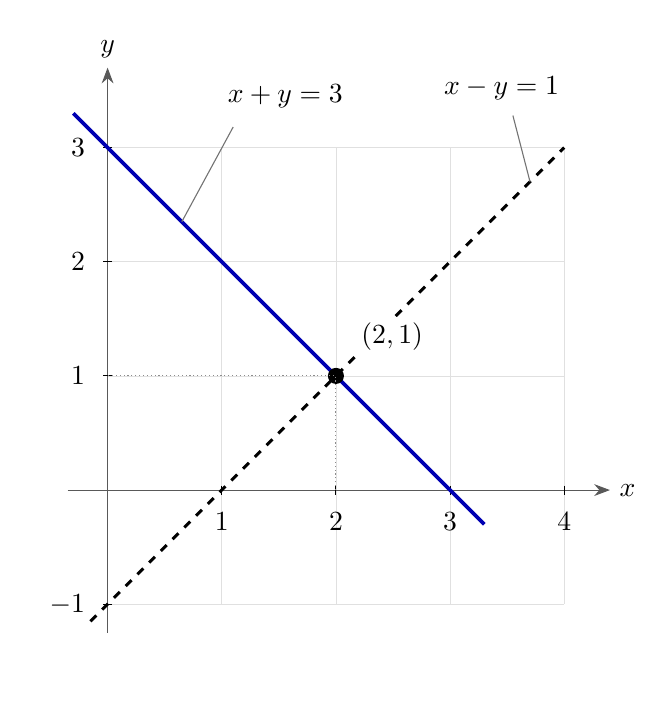
\begin{tikzpicture}[scale=1.45]
\path[use as bounding box] (-.7,-1.65) rectangle (4.65,4.05);
\draw[step=1,black!12,very thin] (0,-1) grid (4,3);
\draw[axis] (-.35,0)--(4.4,0) node[right] {$x$};
\draw[axis] (0,-1.25)--(0,3.7) node[above] {$y$};
\foreach \t in {1,2,3,4} {\draw (\t,.04)--(\t,-.04) node[below=3pt] {$\t$};}
\foreach \t in {-1,1,2,3} {\draw (.04,\t)--(-.04,\t) node[left=3pt] {$\t$};}
\draw[blue!70!black,line width=1.3pt] (-.3,3.3)--(3.3,-.3);
\draw[black,dashed,line width=1.1pt] (-.15,-1.15)--(4,3);
\node[lab,anchor=west] at (1.0,3.45) {$x+y=3$};
\draw[black!55,thin] (1.1,3.18)--(.65,2.35);
\node[lab] at (3.45,3.52) {$x-y=1$};
\draw[black!55,thin] (3.55,3.28)--(3.7,2.7);
\fill (2,1) circle (2pt);
\node[lab,above right=7pt] at (2,1) {$(2,1)$};
\draw[black!45,densely dotted] (2,0)--(2,1)--(0,1);
\end{tikzpicture}
\end{document}
